\documentclass[10pt,a4paper]{article}
\usepackage[utf8]{inputenc}
\usepackage[german]{babel}
\usepackage{mathrsfs}
\usepackage{amsmath}
\usepackage{amsfonts}
\usepackage{amssymb}
\usepackage{amsthm}
\usepackage{graphicx}
\usepackage{float}
\usepackage[left=2cm,right=2cm,top=2cm,bottom=2cm]{geometry}

\begin{document}

\section{Aufgabe 17}
Wenn $n \in \mathbb{N}_{0}$ 0 ist, ist $g_{0}$ die Nullfunktion, die ich nicht zeichne.
\begin{figure}[H]
  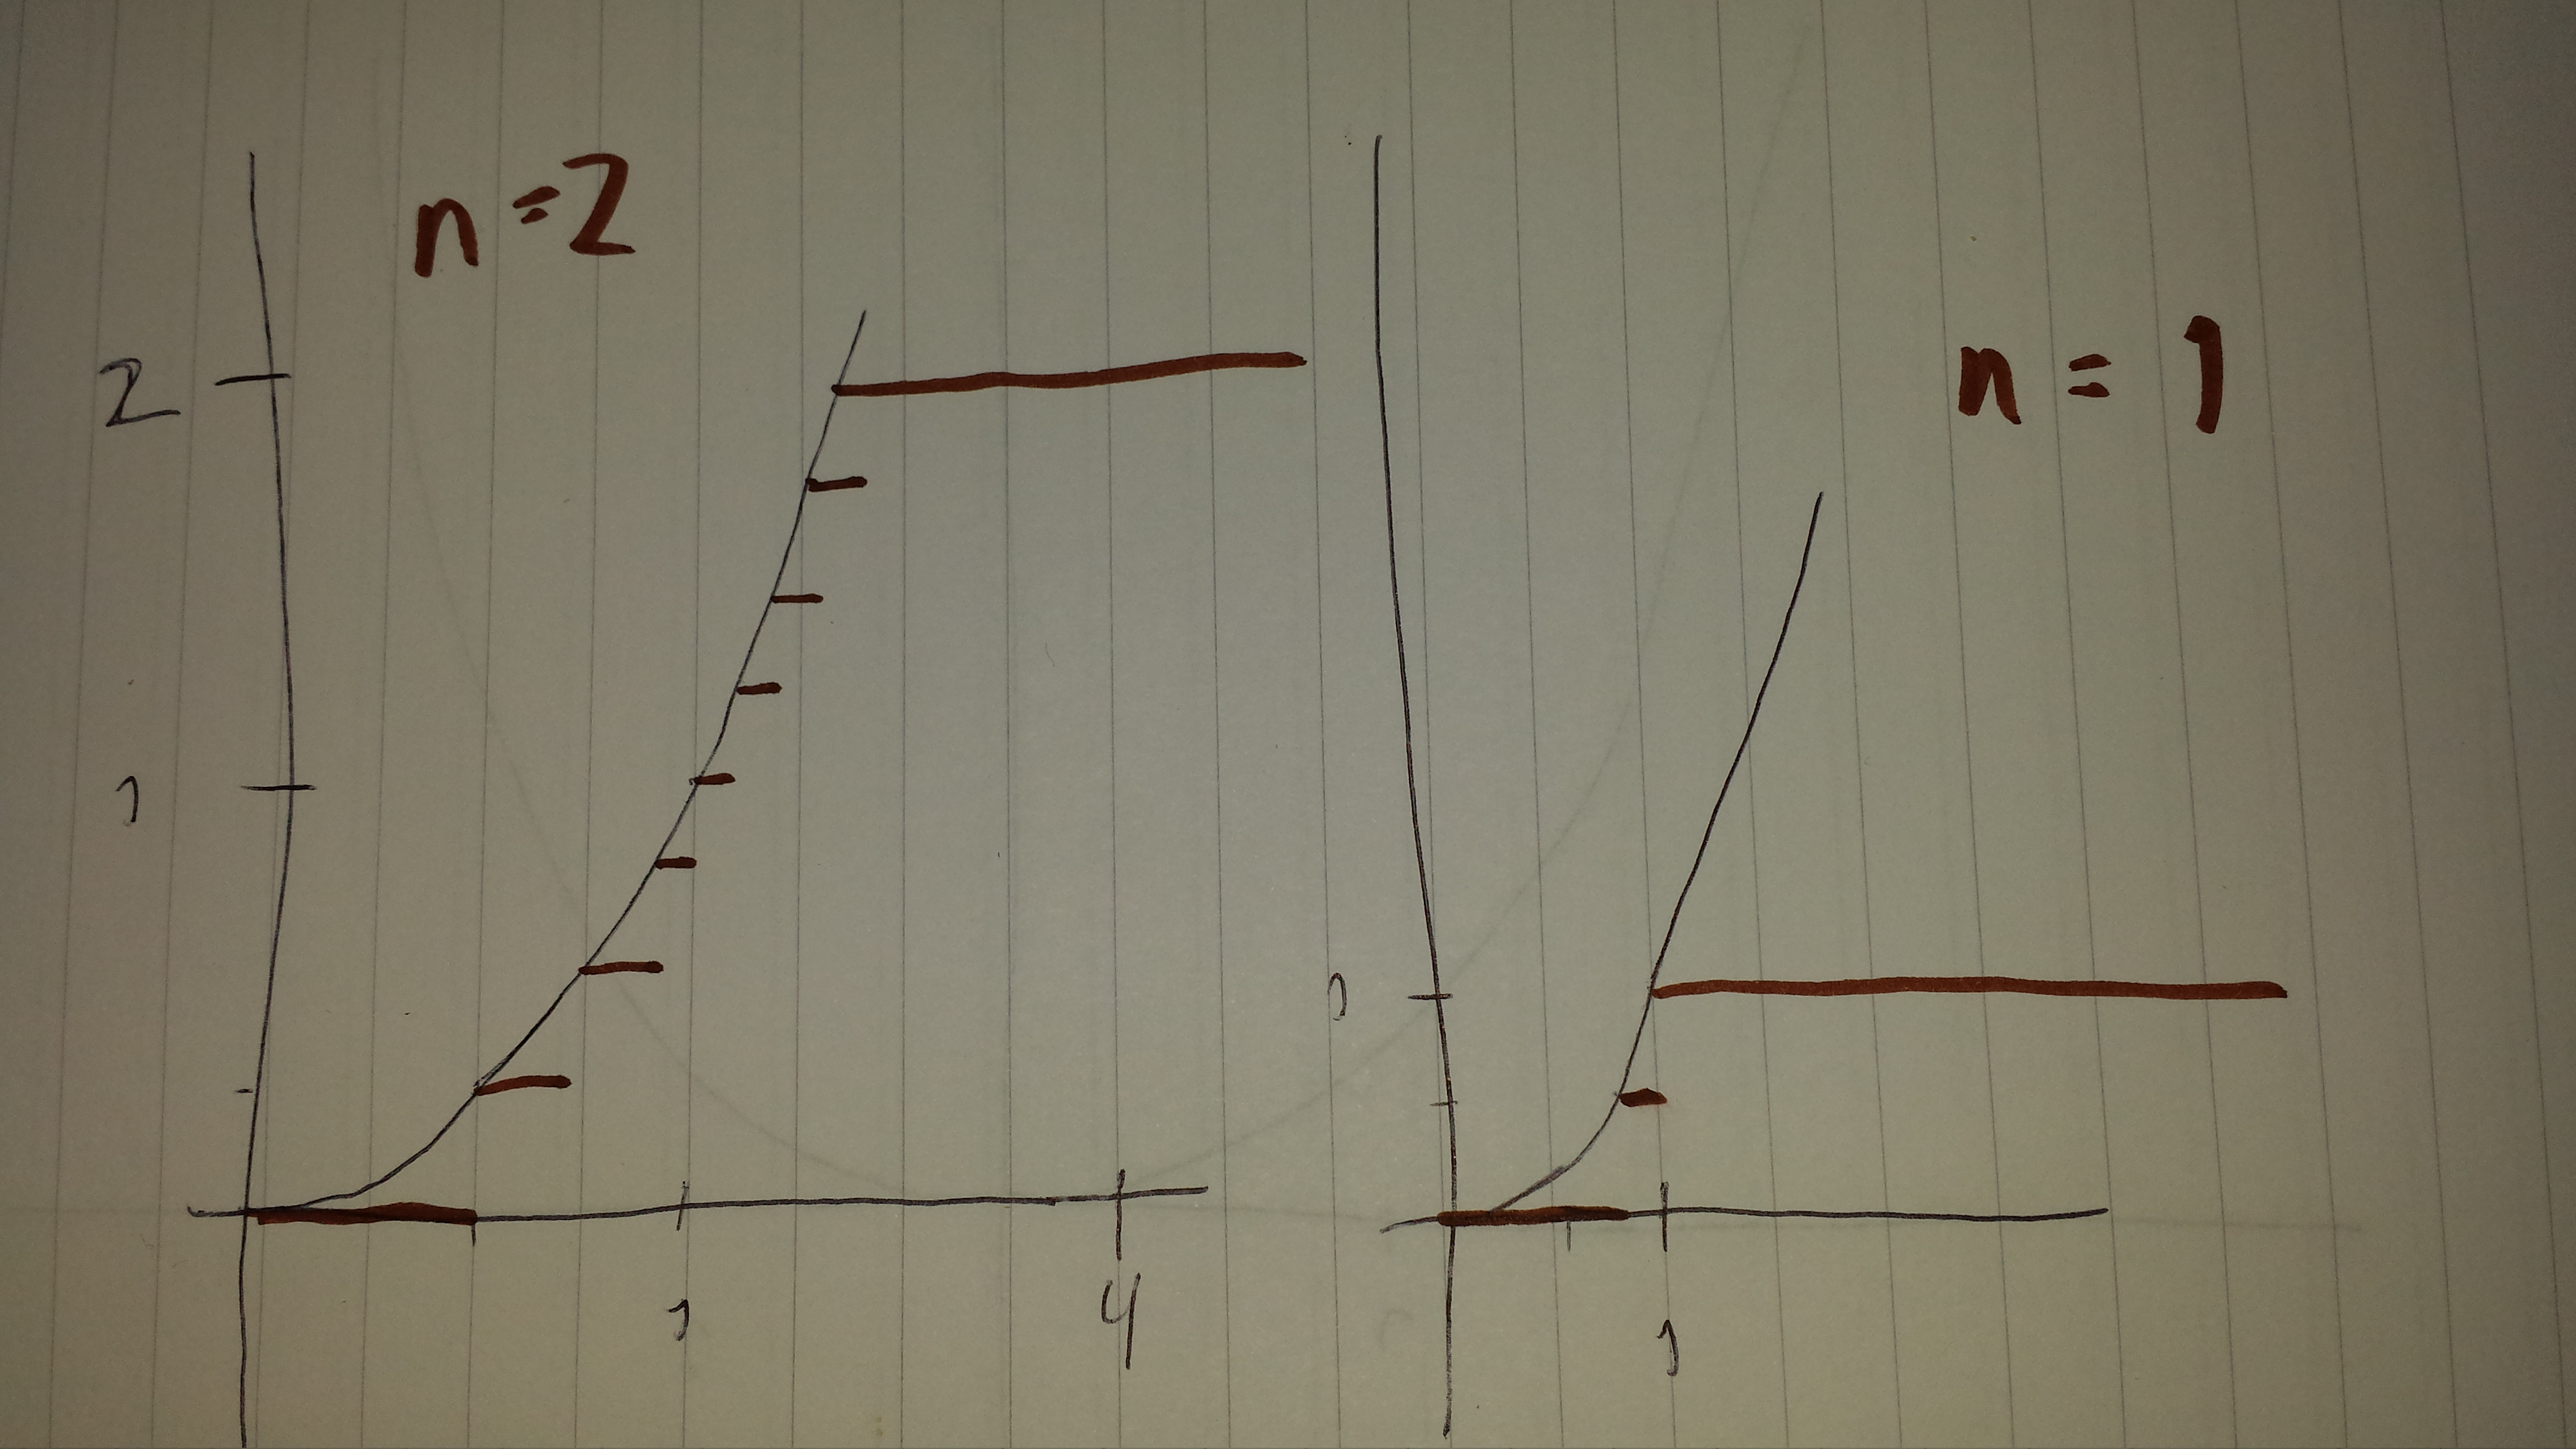
\includegraphics[width=400pt]{5_1}
\end{figure}
Auf den Zeichnungen habe ich es nicht so gut hinbekommen, aber die Stufen werden immer kürzer (außer der letzten).
Und ich habe hier nur die positive Hälfte gezeichnet.
Eigentlich ist es natürlich an der Y-Achse gespiegelt.

\section{Aufgabe 18}

\subsection{Teil a}

\subsection{Teil b}

\subsection{Teil c}
\begin{proof}
  $\Rightarrow$: Sei $lim_{n \rightarrow \infty} a_{n} = a$.
  Nach Definition gibt es für jedes $\epsilon$ ein $n$, sodass $|a_{k} - a| < \frac{\epsilon}{2} \Leftrightarrow -\frac{\epsilon}{2} < a_{k} - a < \frac{\epsilon}{2}$ für alle $k \ge n$.
  Dann ist
  \begin{align*}
    & a - \epsilon < \inf \{ a_{k} \mid k \ge n \} \le \sup \{ a_{k} \mid k \ge n \} < a + \epsilon\\
    \Leftrightarrow & -\epsilon < \inf \{ a_{k} \mid k \ge n \} - a \le \sup \{ a_{k} \mid k \ge n \} - a < \epsilon\\
    \Leftrightarrow & -\epsilon < \inf \{ a_{k} \mid k \ge n \} - a \le \sup \{ a_{k} \mid k \ge n \} - a < \epsilon\\
    \Leftrightarrow & |\inf \{ a_{k} \mid k \ge n \} - a| < \epsilon\ \land\ |\sup \{ a_{k} \mid k \ge n \} - a| < \epsilon\\
    \Leftrightarrow & \liminf_{n \rightarrow \infty} a_{n} = a = \limsup_{n \rightarrow \infty} a_{n}
  \end{align*}
  Die andere Richtung ist einfach rückwärts.
\end{proof}

\subsection{Teil d}

\section{Aufgabe 19}
Sei
\begin{equation}
  f_{n}(x) = 
  \begin{cases}
    & 1\textit{ wenn $x = \frac{2 \cdot k - 1}{2^{n}}$ für ein $k \in [1, 2^{n - 1}]$}\\
    & 0\textit{ sonst}
  \end{cases}
\end{equation}
Dann sind für jedes $n$ alle jeweils Zähler und Nenner der 1-Stellen teilerfremd, weil der Nenner nur durch 2 teilbar ist, der Zähler jedoch nie.
Also sind die Koordinaten der 1-Stellen nicht kürzbar.
Das bedeutet, dass keine zwei $f_{p}$ und $f_{q}$ mit $p \ne q$ eine gemeinsame 1-Stelle haben, da sich sonst die Koordinate der einen 1-Stelle zur Koordinate der anderen 1-Stelle kürzen lassen müsste.
Für jedes $x \in [0, 1]$ gibt es also höchstens ein $f_{n}$ mit $f_{n}(x) = 1$.
Somit ist die Summe aller $f_{n}$ durch 1 beschränkt.
Da alle $f_{n}$ nicht negativ sind, konvergiert die Summe deshalb auch.
Außerdem sind alle $f_{n}$ Riemann-integrierbar, weil sie Treppenfunktionen im riemannschen Sinne sind: Es gibt endlich viele 0-Stufen und ebenfalls nur endlich viele einpunktige Ausnahmen.
$f$ ist jedoch nicht Riemann-integrierbar, weil die eingrenzenden Treppenfunktionen die 0-Funktion und die 1-Funktion sind (genau genommen nur Stufen mit den Werten 0 und 1 haben können).
\begin{proof}
  Da $f$ nur abzählbar viele 1-Stellen hat, kann keine untere Treppenfunktion größer als die 0-Funktion sein.

  Sei $g$ eine obere Treppenfunktion und $]a, b[$ eine Stufe von $g$ auf der $g$ einen Wert kleiner als 1 annimmt.
  Dann sind $0 \le a < b \le 1$.
  Dann gibt es ein $n$ für das $f_{n}$ auf $]a, b[$ eine 1-Stelle besitzt und somit auch $f$, sodass $g$ keine obere Treppenfunktion von $f$ sein kann.
  Da die 1-Stellen von $f_{n}$ einen Abstand von $\frac{2}{2^{n}}$ haben, muss folgendes gelten
  \begin{equation}
    \frac{2}{2^{n}} < a - b \Leftrightarrow \frac{2}{a - b} < 2^{n} \Leftrightarrow n > \log_{2}(\frac{2}{a - b})
  \end{equation}
  Sei also $n = \lceil \log_{2}(\frac{2}{a - b}) \rceil + 1$.
  Dann gibt es mindestens ein $x \in ]a, b[$ mit $f_{n}(x) = 1$.
\end{proof}

\section{Aufgabe 20}
\begin{proof}
  Sei $P = \{ x \in X \mid f(x) = \pm \infty \}$.
  Um zu zeigen, dass $f$ fast überall endlich ist, ist also zu zeigen, dass $\mu(P) = 0$.
  Ich beweise es per Widerspruch.
  Angenommen $\mu(P) > 0$.
  Da $f$ integrierbar ist, sind $\int f^{+} d\mu$ und $\int f^{-} d\mu$ endlich.
  Dann ist $P^{+} = \{ x \in X \mid f(x) = +\infty \}$ und $P^{-} = \{ x \in X \mid f(x) = -\infty \}$ eine disjunkte Aufteilung von $P$.
  Deswegen ist mindestens $\mu(P^{+}) > 0$ oder $\mu(P^{-}) > 0$, vielleicht auch beides.
  O.b.d.A. nehme ich an, dass $\mu(P^{+}) > 0$.
  Wenn das nicht der Fall ist, gilt die Argumentation genauso für $P^{-}$ und $f^{-}$.
  Dann ist $f^{+}(x) = \infty\ \forall x \in P^{+}$.
  Nach Definition des Integrals gibt es eine wachsende Folge $(g_{n})$ von Treppenfunktionen mit $f^{+} = \sup_{n} g_{n}$.
  Sei $a_{n}$ das Minimum der Werte, die $g_{n}$ auf $P^{+}$ annimmt.
  \begin{equation}
    \int f^{+} d\mu = \sup_{n} \int g_{n} d\mu \ge \sup_{n} a_{n} \cdot \mu(P^{+}) = \mu(P^{+}) \cdot \sup_{n} a_{n} = \mu(P^{+}) \cdot \infty = \infty
  \end{equation}
  Aber dies widerspricht der Endlichkeit von $\int f^{+} d\mu$, sodass $\mu(P) = 0$ sein muss.
\end{proof}

\section{Aufgabe 21}
\begin{equation}
  f_{n}(x) = 
  \begin{cases}
    & 1\textit{ wenn $n \le x \le n + 1$}\\
    & 0\textit{ sonst}
  \end{cases}
\end{equation}
\begin{equation}
  g_{n}(x) = 
  \begin{cases}
    & 2\textit{ wenn $n \le x \le n + 1$}\\
    & 0\textit{ sonst}
  \end{cases}
\end{equation}
Dann konvergieren bei Folgen gegen die $0$-Funktion, weil es für jedes $x$ ein $N$ gibt, sodass $f_{n}(x) = g_{n}(x) = 0$ für alle $n \ge N$.
Allerdings ist $\lim_{n \rightarrow \infty} \int f_{n} d \lambda^{1} = 1$ und $\lim_{n \rightarrow \infty} \int g_{n} d \lambda^{1} = 2$.

\end{document}